% !TEX root = SystemTemplate.tex

\chapter{Overview and concept of operations}

%The overview should take the form of an executive summary.  Give the reader a feel 
%for the purpose of the document, what is contained in the document, and an idea 
%of the purpose for the system or product. 


\section{Scope}
%What scope does this document cover? 
The scope of this document is meant to cover the process, organization,
technologies, and documentation for the creation of the program
Program Tester (stage 1)

\section{Purpose}
%What is the purpose of the system or product? 
The purpose of this program is to run test files on another
 program and record the results in a log file.

It accomplishes this by being placed in the directory to traverse. Once run it will traverse into each student directory and run the program against all the tests in the the tests sub-directory. Before this however, the user has to option to have the test suite generate the test documents.

\section{Sprint 1}

\subsection{Major System Component \#1}
Locate cpp file and compile it.

\subsection{Major System Component \#2}
Find test files and run them on the program.

\subsection{Major System Component \#3}
Record the results in a log file.

\section{Sprint 2}

\subsection{Major System Component \#4}
Locate the cpp file and compile it for each student in the class.

\subsection{Major System Component \#5}
Create an individual log file that has the results of the test cases run against
that student's executable. Only if all critical tests are passed will the student's
executable be run against the rest of the test cases. Log all of the final results
for each student in a class summary log file in the main directory.

\subsection{Major System Component \#6}
Automatically generate test cases for either floats or ints. The type of test cases
and number of test cases generated are determined by user input.

\section{Systems Goals}
%Briefly describe the overall goals this system plans to achieve.  These goals are 
%typically provided by the stakeholders.  This is not intended to be a detailed 
%requirements listing.  Keep in mind that this section is still part of the Overview.
This project will check all sub-directories for cpp files. Each sub-directory
belongs to a student and contains their cpp file. These files are individually
compiled. They will each be run against test cases, first the critical tests and
provided those pass then the rest of the test files. The results of each test case
are written in the student's log file. The final results of each student's
performance will be written in a class summary log file. The user will be able
to have test cases automatically generated for either floats or ints. This project
was created for the use of computer science professors to aid in the grading of
their student's programs.
%\section{System Overview and Diagram}
%Provide a more detailed description of the major system components without getting 
%too detailed.  This section should contain a high-level block and/or flow diagram 
%of the system highlighting the major components.   See Figure~\ref{systemdiagram}.    This is a floating figure environment.  \LaTeX\ will try to put it close %to where it was typeset but will not allow the figure to be split if moving it can not happen.   Figures, tables, algorithms and many other floating %environments are automatically numbered and placed in the appropriate type of table of contents.  You can move these and the numbers will update %correctly.

%\begin{figure}[tbh]
%\begin{center}
%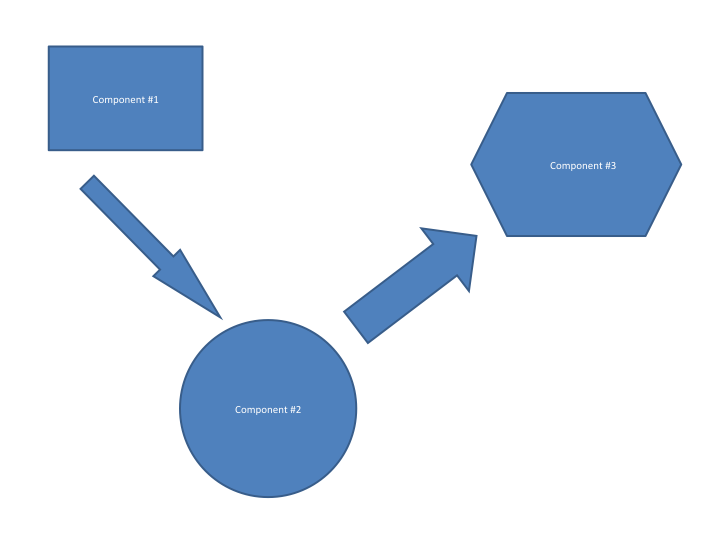
\includegraphics[width=0.75\textwidth]{./diagram}
%\end{center}
%\caption{A sample figure .... System Diagram \label{systemdiagram}}
%\end{figure}

\section{Technologies Overview}
%This section should contain a list of specific technologies used to develop the 
%system.  The list should contain the name of the technology, brief description, 
%link to reference material for further understanding, and briefly how/where/why 
%it was used in the system.    See Table~\ref{somenumbers}.  This is a floating table environment.  \LaTeX\ will try to put it close to where it was typeset but %will not allow the table to be split.   
%\begin{table}[tbh]
%\begin{center}
%\begin{tabular}{|r|l|}
  %\hline
  %7C0 & hexadecimal \\
  %3700 & octal \\ \cline{2-2}
  %11111000000 & binary \\
  %\hline \hline
  %1984 & decimal \\
  %\hline
%\end{tabular}
%\caption{A sample Table ... some numbers. \label{somenumbers}}
%\end{center}
%\end{table}
This project was created using an x86 processor running Fedora 20 linux. It was
compiled and compiles using the g++ compiler. It was developed using the Agile
Scrum development method. A Trello board was used to track the progress of the
project. A Git repository was used for the version control of this project. The
documentation was created using LateX.
